\chapter{The Higgs Mechanism: How a Gauge Boson Acquires Mass}

We now join the two ideas developed in the previous lecture. A complex scalar
field with a broken global \(U(1)\) symmetry contains a massive radial
oscillation and a massless angular oscillation. A locally invariant \(U(1)\)
theory contains a massless gauge field. When the scalar is charged and its
equilibrium magnitude is nonzero, these statements cannot simply be added
together. The angular mode and the gauge field combine: the gauge field
becomes massive, the apparent Goldstone boson ceases to be an independent
particle, and the radial Higgs mode remains.

The photon will be our model gauge boson, but not our physical conclusion.
Electromagnetic \(U(1)\) is not broken in the vacuum, so the real photon is
massless. The same mechanism acts on the \(W^\pm\) and \(Z\) in the
electroweak theory, where the gauge group and scalar multiplet are more
complicated. The abelian model exposes the mechanism without hiding it under
group theory.

\begin{classroomqa}
\audiencequestion{Did the previous discussion mean that the Higgs mechanism
gives a mass to the real photon?\lecturetimestamp{00:00:23}}
\lecturerresponse{No. We ask what would happen \emph{if} the \(U(1)\)
associated with the photon were in a broken phase. That hypothetical photon
would become massive. The real electromagnetic vacuum is not in that phase;
the application to particle physics is instead the mass of the \(W\) and
\(Z\).}
\end{classroomqa}

The symmetry associated with electric-charge conservation is the phase
rotation
\begin{equation}
  \phi(x)\longmapsto e^{i\theta}\phi(x),
\end{equation}
an internal rotation called \(U(1)\). A superconductor provides a real
analogue of the broken phase. Inside it, the electromagnetic field has a
finite penetration depth and behaves in important respects like a massive
field. Outside it, the ordinary massless photon reappears.

\section{What Mass Means for a Field}

\subsection{Dispersion and the zero-momentum gap}

It is worth deciding precisely what we mean by mass before introducing the
Higgs field. For a wave,
\begin{equation}
  E=\hbar\omega,
  \qquad
  p=\hbar k,
  \label{eq:l08-quantum-wave}
\end{equation}
so an \((E,p)\) graph and an \((\omega,k)\) graph contain the same
information up to factors of \(\hbar\). In empty space a massless
relativistic excitation obeys
\begin{equation}
  E=c|p|,
  \qquad
  \omega=c|k|.
  \label{eq:l08-massless-dispersion}
\end{equation}
The two signs of \(k\) distinguish opposite directions of propagation. The
essential point is that \(\omega\) tends to zero with \(k\).

A massive relativistic particle obeys
\begin{equation}
  E^2=c^2p^2+m^2c^4.
  \label{eq:l08-massive-dispersion}
\end{equation}
In units \(c=\hbar=1\),
\begin{equation}
  \omega^2=k^2+m^2.
\end{equation}
At \(k=0\), the energy is \(E=mc^2\), or simply \(m\) in natural units.
Thus mass is the nonzero energy gap of the zero-momentum mode.

\begin{figure}[htbp]
\centering
\begin{adjustbox}{max width=\linewidth}
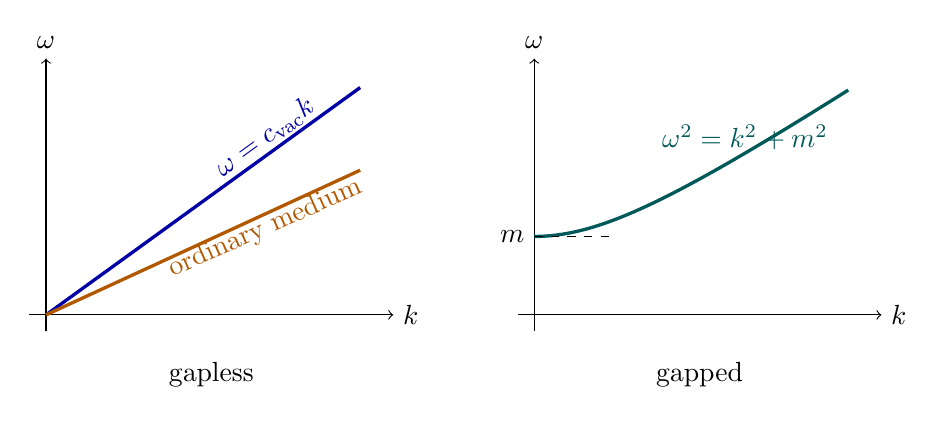
\begin{tikzpicture}[x=1.05cm,y=1.05cm]
  \begin{scope}
    \draw[->] (-0.2,0) -- (4.2,0) node[right] {\(k\)};
    \draw[->] (0,-0.2) -- (0,3.1) node[above] {\(\omega\)};
    \draw[very thick,blue!65!black] (0,0) -- (3.8,2.75);
    \draw[very thick,orange!70!black] (0,0) -- (3.8,1.75);
    \node[blue!65!black,rotate=36] at (2.65,2.15)
      {\(\omega=c_{\rm vac}k\)};
    \node[orange!70!black,rotate=24] at (2.65,1.05)
      {ordinary medium};
    \node[below] at (2,-0.45) {gapless};
  \end{scope}
  \begin{scope}[xshift=6.2cm]
    \draw[->] (-0.2,0) -- (4.2,0) node[right] {\(k\)};
    \draw[->] (0,-0.2) -- (0,3.1) node[above] {\(\omega\)};
    \draw[very thick,domain=0:3.8,samples=120,smooth,teal!70!black]
      plot (\x,{sqrt(0.9+0.45*\x*\x)});
    \draw[dashed] (0,0.95) -- (1.0,0.95);
    \node[left] at (0,0.95) {\(m\)};
    \node[teal!70!black] at (2.55,2.15)
      {\(\omega^2=k^2+m^2\)};
    \node[below] at (2,-0.45) {gapped};
  \end{scope}
\end{tikzpicture}
\end{adjustbox}
\caption{Changing the propagation speed changes the slope of a gapless
dispersion relation. Giving the excitation a mass opens a nonzero gap at
\(k=0\).}
\label{fig:l08-dispersion}
\end{figure}

An ordinary transparent material may lower a wave's phase velocity without
creating this relativistic mass gap. At a boundary the incident frequency is
fixed, while the wave number adjusts to the medium's dispersion relation.
Changing the slope is not the same as lifting the intercept.
\editorialnote{A material can have several electromagnetic branches, and a
plasma or resonant medium can possess a nonzero plasma-frequency gap. The
lecture's comparison is specifically between an ordinary refractive branch
and the superconducting response. More generally, gaplessness means
\(\omega(k)\to0\) as \(k\to0\); exact linearity is not required in every
nonrelativistic medium.}

\begin{classroomqa}
\audiencequestion{Does a photon acquire mass whenever it travels through
matter, for example through a prism?\lecturetimestamp{00:03:02}}
\lecturerresponse{No. Refraction can change the relation between frequency
and wave number, and therefore the propagation speed, while the branch still
passes through \(\omega=0\) at \(k=0\). A superconducting phase instead gives
the electromagnetic response a finite inverse penetration length, the
analogue of a mass.}
\end{classroomqa}

\begin{classroomqa}
\audiencequestion{For light of a fixed frequency entering glass, is it the
wave number that changes?\lecturetimestamp{00:09:20}}
\lecturerresponse{Yes. Time-translation invariance at a stationary interface
keeps the frequency fixed. Because the dispersion curve has a different
slope in the glass, the same \(\omega\) corresponds to a different \(k\), and
therefore a different wavelength.}
\end{classroomqa}

The slope
\begin{equation}
  v_g=\frac{d\omega}{dk}
\end{equation}
is the group velocity of a wave packet. If that slope varies with \(k\),
different Fourier components move at different speeds and the packet
disperses. This is why the relation \(\omega(k)\) is called the
\emph{dispersion relation}.

\begin{classroomqa}
\audiencequestion{What is the name of the curve, and what does its slope
represent?\lecturetimestamp{00:11:02}}
\lecturerresponse{The curve is the dispersion relation. Its derivative
\(d\omega/dk\) is the group velocity. A constant slope gives the same velocity
to all wavelengths; a varying slope makes a wave packet spread. For the
present purpose, the decisive distinction is whether the curve reaches the
origin or has a gap.}
\end{classroomqa}

\subsection{A homogeneous oscillation is a particle at rest}

The mode \(k=0\) has infinite wavelength: the field is displaced by the same
amount everywhere. Release a homogeneous displacement. If the field
oscillates with a nonzero frequency, the corresponding quantum has a nonzero
rest energy and is massive. If there is no restoring force in that direction,
the frequency vanishes and the mode is massless.

This statement is classical. It does not require spatially separated
particles to be in a quantum superposition. A homogeneous classical field
configuration is simply one field value repeated throughout space.

\begin{classroomqa}
\audiencequestion{If an entire field is shifted together, is that the same as
quantum entanglement?\lecturetimestamp{00:10:04}}
\lecturerresponse{No. A homogeneous classical field is one classical
configuration. Entanglement correlates distinct quantum alternatives, such
as up--down and down--up spin configurations. Preparing the same field value
at many points is not by itself entanglement, nor does it imply an
instantaneous causal response.}
\end{classroomqa}

For a canonically normalized real field,
\begin{equation}
  \mathcal L
  =\frac12\partial_\mu\varphi\,\partial^\mu\varphi-V(\varphi),
\end{equation}
expand about an equilibrium \(\varphi_0\):
\begin{equation}
  V(\varphi_0+\eta)
  =V(\varphi_0)
   +\frac12V''(\varphi_0)\eta^2+\cdots.
\end{equation}
The linear term vanishes at the minimum, and the field equation gives
\begin{equation}
  \omega^2=\bm{k}^2+m^2,
  \qquad
  m^2=V''(\varphi_0).
  \label{eq:l08-curvature-mass}
\end{equation}
Mass is therefore the curvature of the potential in the direction of
motion. A flat direction has zero curvature and yields a massless mode.

\section{The Broken Complex Scalar}

\subsection{Radial and angular motion}

Write a complex scalar in Cartesian and polar coordinates:
\begin{equation}
  \phi=\phi_R+i\phi_I=\rho e^{i\alpha},
  \qquad
  \phi^*=\phi_R-i\phi_I=\rho e^{-i\alpha}.
  \label{eq:l08-polar-field}
\end{equation}
The complex plane is an \emph{internal} field space. At every physical
spacetime point \(x\), the pair
\((\phi_R(x),\phi_I(x))\) specifies one point in that internal plane.
Neither internal axis is a direction in the laboratory.

\begin{figure}[htbp]
\centering

\includegraphics[width=0.72\textwidth]{lecture_08_figure_02.png}
\caption{The complex scalar represented in its internal
\((\phi_R,\phi_I)\)-plane. The radius is \(\rho\), and \(\alpha\) is the
internal phase.}
\lectureframe{00:24:41}
\label{fig:l08-internal-plane}
\end{figure}

The scalar kinetic term becomes
\begin{align}
  \partial_\mu\phi^*\,\partial^\mu\phi
  &=
  \partial_\mu\phi_R\,\partial^\mu\phi_R
  +\partial_\mu\phi_I\,\partial^\mu\phi_I
  \notag\\
  &=
  \partial_\mu\rho\,\partial^\mu\rho
  +\rho^2\partial_\mu\alpha\,\partial^\mu\alpha.
  \label{eq:l08-polar-kinetic}
\end{align}
A globally \(U(1)\)-invariant potential depends on
\(\phi^*\phi=\rho^2\), not on \(\alpha\). For example,
\begin{equation}
  V(\phi)
  =\lambda\left(\phi^*\phi-\frac{f^2}{2}\right)^2,
  \qquad \lambda>0.
  \label{eq:l08-mexican-hat}
\end{equation}
Its minima form a circle. The law is invariant under a common phase
rotation, but choosing one equilibrium phase selects one point on the
circle.

\begin{figure}[htbp]
\centering

\includegraphics[width=0.78\textwidth]{lecture_08_figure_03.png}
\caption{The board's radial potential sketches. The potential is symmetric
under rotations of the internal field value, even though the field itself
need not sit at the origin.}
\lectureframe{00:34:22}
\label{fig:l08-radial-potential-board}
\end{figure}

\begin{figure}[htbp]
\centering
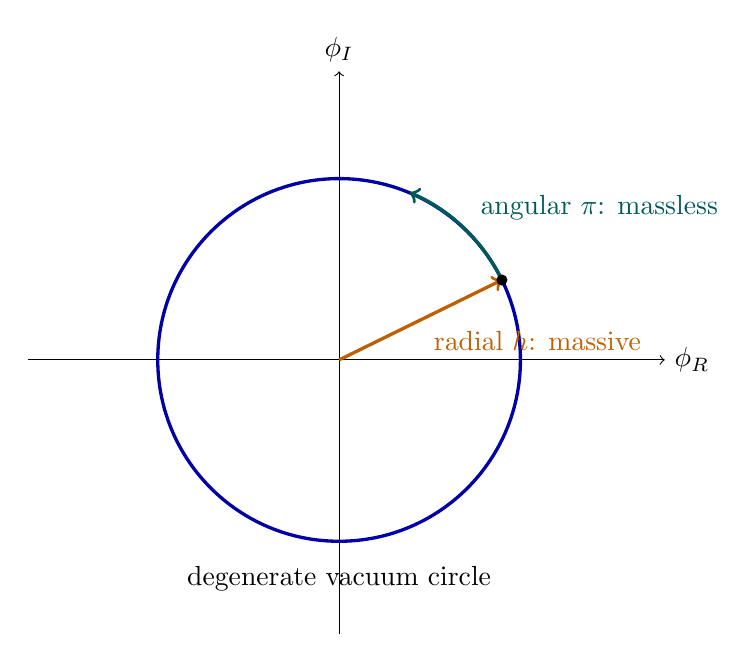
\begin{tikzpicture}[x=0.94cm,y=0.94cm]
  \draw[->] (-4.2,0) -- (4.4,0) node[right] {\(\phi_R\)};
  \draw[->] (0,-3.7) -- (0,3.9) node[above] {\(\phi_I\)};
  \draw[very thick,blue!65!black] (0,0) circle (2.45);
  \draw[->,very thick,orange!75!black] (0,0) -- (2.2,1.08);
  \draw[->,very thick,teal!70!black]
    (2.2,1.08) arc[start angle=26,end angle=67,radius=2.45];
  \node[orange!75!black,below right] at (1.15,0.52)
    {radial \(h\): massive};
  \node[teal!70!black,above right] at (1.78,1.76)
    {angular \(\pi\): massless};
  \fill (2.2,1.08) circle (2pt);
  \node[below] at (0,-2.65) {degenerate vacuum circle};
\end{tikzpicture}
\caption{The global broken theory has curvature normal to the vacuum circle
but no curvature along it. The radial Higgs mode is massive; the angular
Goldstone mode is massless.}
\label{fig:l08-radial-angular}
\end{figure}

Set
\begin{equation}
  \phi(x)=\frac{f+h(x)}{\sqrt2}
           e^{i\pi(x)/f}.
  \label{eq:l08-canonical-polar}
\end{equation}
Near the selected vacuum, \(h\) measures radial displacement and \(\pi\)
measures tangential displacement with canonical dimensions. Substitution in
Eq.~\eqref{eq:l08-polar-kinetic} gives
\begin{equation}
  \partial_\mu\phi^*\,\partial^\mu\phi
  =
  \frac12(\partial_\mu h)^2
  +\frac12\left(1+\frac{h}{f}\right)^2
            (\partial_\mu\pi)^2.
  \label{eq:l08-global-expanded}
\end{equation}
The potential in Eq.~\eqref{eq:l08-mexican-hat} supplies
\begin{equation}
  m_h^2=2\lambda f^2,
  \qquad
  m_\pi^2=0.
  \label{eq:l08-global-masses}
\end{equation}
At energies far below \(m_h\), radial motion is expensive, so we may
temporarily freeze \(h=0\). The remaining Lagrangian contains only
\(\frac12(\partial\pi)^2\), with no \(\pi^2\) term. This is the Goldstone
boson.\editorialnote{At two points the spoken explanation reverses the names and
says that eating the Goldstone gives the Higgs boson its mass. The board
calculation and the remainder of the lecture establish the intended result:
radial curvature already gives the Higgs mode a mass, while the gauge boson
acquires the Goldstone mode and becomes massive.}

\begin{classroomqa}
\audiencequestion{Is this the only spontaneous symmetry breaking in the
Standard Model?\lecturetimestamp{00:16:39}}
\lecturerresponse{The electroweak Higgs phase is the established
symmetry-breaking mechanism relevant here. Its actual symmetry is
\(SU(2)_L\times U(1)_Y\), not this single \(U(1)\), and QCD has additional
vacuum structure such as chiral symmetry breaking. The abelian example is a
deliberately reduced model of the gauge-boson mechanism.}
\end{classroomqa}

\begin{classroomqa}
\audiencequestion{Does the Higgs give mass to every particle, including
itself?\lecturetimestamp{00:17:11}}
\lecturerresponse{There is a yes-and-no distinction. Electroweak symmetry
forbids bare masses for the \(W\), \(Z\), and Standard Model fermions; their
masses appear after the Higgs field takes a nonzero equilibrium magnitude.
The radial Higgs mass comes from the curvature of its own potential. Other
hypothetical particles can possess symmetry-allowed masses unrelated to this
mechanism.}
\end{classroomqa}

The lecture associates such symmetry-allowed masses with potentially very
heavy, difficult-to-observe particles and mentions dark matter as a possible
example. That is a motivation, not a mass prediction.
\editorialnote{The dark-matter mass scale remains unknown. The lecture's
suggestion of a particle around a thousand proton masses is historical
speculation, not an experimentally established property of dark matter.}

\begin{classroomqa}
\audiencequestion{Is \(\rho\) a physical radius, or is it the field value?
What exactly is radially symmetric?\lecturetimestamp{00:33:08}}
\lecturerresponse{At each spacetime point the field value is a point in an
auxiliary complex plane, and \(\rho=|\phi|\) is the distance of that point
from the origin. The \emph{potential} is radially symmetric in this internal
plane: all points with the same \(\rho\) have the same potential energy.
This radius is not a distance in ordinary space.}
\end{classroomqa}

\begin{classroomqa}
\audiencequestion{Could a sufficiently violent radial kick carry the field
over the central maximum to the other side of the potential?
\lecturetimestamp{00:36:00}}
\lecturerresponse{In principle a local configuration with enough energy can
cross the barrier. Moving a homogeneous macroscopic field over it would
require an enormous energy, and a generic violent disturbance would shed
energy into many field modes rather than arrive coherently at the opposite
point. The low-energy approximation freezes \(\rho\) precisely because such
radial excursions are inaccessible there.}
\end{classroomqa}

\section{Why the Complex Plane Is Not Spacetime}

The distinction between physical and internal coordinates deserves the
lecture's full pause. A scalar field is called scalar because it is invariant
under rotations of physical coordinate axes. Two real scalar fields
\(\phi_R(x)\) and \(\phi_I(x)\) remain two scalars under those rotations. We
may package them into one complex number, but this bookkeeping does not turn
them into components of a spatial vector.

A global \(U(1)\) transformation rotates the \emph{values} of the field:
\begin{equation}
\begin{aligned}
  \phi(x)&\longmapsto e^{i\theta}\phi(x),
  \\
  \rho(x)&\longmapsto\rho(x),
  \\
  \alpha(x)&\longmapsto\alpha(x)+\theta.
\end{aligned}
  \label{eq:l08-global-shift}
\end{equation}
The same constant \(\theta\) is used at every spacetime point. Consequently,
\(\partial_\mu\alpha\) is unchanged. This is a symmetry of both the potential
and the ordinary kinetic term. Once \(\theta\) is allowed to depend on
\(x\), the derivative detects the variation, and the argument changes.

\section{Making the Phase Rotation Local}

\subsection{The ordinary derivative fails}

Let
\begin{equation}
  \phi'(x)=e^{i\theta(x)}\phi(x).
  \label{eq:l08-local-phase}
\end{equation}
Then
\begin{equation}
  \partial_\mu\phi'
  =e^{i\theta}
    \left(\partial_\mu\phi+i\,\partial_\mu\theta\,\phi\right).
  \label{eq:l08-ordinary-derivative-fails}
\end{equation}
The extra term proportional to \(\partial_\mu\theta\) prevents
\(\partial_\mu\phi\) from transforming like \(\phi\). Therefore
\(\partial_\mu\phi^*\partial^\mu\phi\) is not invariant under arbitrary local
phase rotations.

\begin{figure}[htbp]
\centering

\includegraphics[width=0.78\textwidth]{lecture_08_figure_04.png}
\caption{The board records the local phase transformation and the failure of
the ordinary derivative term to remain invariant.}
\lectureframe{00:46:49}
\label{fig:l08-local-not-symmetry}
\end{figure}

Introduce a vector potential and fix one convention consistently:
\begin{equation}
  D_\mu=\partial_\mu+i g A_\mu,
  \qquad
  A_\mu'=A_\mu-\frac1g\partial_\mu\theta.
  \label{eq:l08-covariant-convention}
\end{equation}
Now
\begin{align}
  D_\mu'\phi'
  &=
  \left(\partial_\mu+i g A_\mu'\right)
  e^{i\theta}\phi
  \notag\\
  &=
  e^{i\theta}
  \left[
    \partial_\mu\phi+i(\partial_\mu\theta)\phi
    +i g A_\mu\phi-i(\partial_\mu\theta)\phi
  \right]
  \notag\\
  &=e^{i\theta}D_\mu\phi.
  \label{eq:l08-covariant-transform}
\end{align}
The unwanted terms cancel. The conjugate derivative is
\begin{equation}
  (D_\mu\phi)^*
  =(\partial_\mu-i g A_\mu)\phi^*,
\end{equation}
and its opposite phase cancels in the product
\begin{equation}
  (D_\mu\phi)^*D^\mu\phi.
\end{equation}

\begin{classroomqa}
\audiencequestion{Was the gauge-field transformation written with the
opposite sign in the previous lecture?\lecturetimestamp{00:48:04}}
\lecturerresponse{A simultaneous reversal of the sign in \(D_\mu\) and in
the transformation law is merely a convention. With
\(D_\mu=\partial_\mu+i gA_\mu\) and
\(\phi'=e^{i\theta}\phi\), consistency requires
\(A_\mu'=A_\mu-g^{-1}\partial_\mu\theta\). The alternative convention works
equally well if every sign is changed together.}
\end{classroomqa}

\begin{classroomqa}
\audiencequestion{Does the use of an upper-case or lower-case form of
\(\phi\) on the board mark a different field?\lecturetimestamp{00:55:02}}
\lecturerresponse{No distinction is intended. The changing letter shape is
handwriting, not an additional operation or a second scalar. The meaningful
distinctions are the prime, the complex-conjugation star, and the spacetime
index.}
\end{classroomqa}

\begin{classroomqa}
\audiencequestion{Is complex conjugation the same operation as raising or
lowering the Lorentz index in the kinetic term?
\lecturetimestamp{00:56:50}}
\lecturerresponse{No. The star conjugates the internal complex field.
Lorentz indices are raised with the spacetime metric:
\(D^\mu=g^{\mu\nu}D_\nu\). A Lorentz scalar needs the contraction
\((D_\mu\phi)^*D^\mu\phi\); both operations are present and serve different
purposes.}
\end{classroomqa}

\subsection{The gauge field has its own dynamics}

The field strength
\begin{equation}
  F_{\mu\nu}=\partial_\mu A_\nu-\partial_\nu A_\mu
  \label{eq:l08-field-strength}
\end{equation}
is gauge invariant because the two mixed second derivatives of \(\theta\)
cancel. Its time--space components contain the electric field, and its
space--space components contain the magnetic field. The scalar version of
electrodynamics is therefore
\begin{equation}
  \mathcal L
  =(D_\mu\phi)^*D^\mu\phi
  -V(\phi^*\phi)
  -\frac14F_{\mu\nu}F^{\mu\nu}.
  \label{eq:l08-abelian-higgs}
\end{equation}
The charged field here is bosonic. It is not the electron field, which is a
fermion. A charged helium nucleus or a Cooper-pair condensate illustrates
how a bosonic charged degree of freedom can arise.

Before symmetry breaking, the gauge term contains derivatives of \(A_\mu\)
but no direct mass term. One might try to add
\begin{equation}
  \frac12m_A^2A_\mu A^\mu,
\end{equation}
but under Eq.~\eqref{eq:l08-covariant-convention},
\begin{equation}
  A_\mu A^\mu
  \longmapsto
  \left(A_\mu-\frac1g\partial_\mu\theta\right)
  \left(A^\mu-\frac1g\partial^\mu\theta\right),
  \label{eq:l08-bare-mass-fails}
\end{equation}
which is not equal to \(A_\mu A^\mu\). A bare gauge-boson mass is forbidden
by the local symmetry.

\begin{figure}[htbp]
\centering

\includegraphics[width=0.76\textwidth]{lecture_08_figure_05.png}
\caption{A verified board state for the obstruction: under a gauge
transformation, \(A_\mu A^\mu\) becomes a square containing
\(\partial_\mu\theta\), so a bare vector mass is not invariant.}
\lectureframe{01:07:30}
\label{fig:l08-bare-mass-board}
\end{figure}

\section{The Higgs Mechanism}

\subsection{The covariant derivative produces the mass}

Return to the broken potential and use the canonically normalized
parametrization
\begin{equation}
  \phi(x)=\frac{f+h(x)}{\sqrt2}
  e^{i\pi(x)/f}.
\end{equation}
Its covariant derivative is
\begin{equation}
  D_\mu\phi
  =
  \frac{e^{i\pi/f}}{\sqrt2}
  \left[
    \partial_\mu h
    +i(f+h)
      \left(\frac{\partial_\mu\pi}{f}+gA_\mu\right)
  \right].
  \label{eq:l08-covariant-polar}
\end{equation}
Consequently,
\begin{equation}
\begin{aligned}
  (D_\mu\phi)^*D^\mu\phi
  ={}&
  \frac12(\partial_\mu h)^2
  \\
  &+\frac12(f+h)^2
    \left(\frac{\partial_\mu\pi}{f}+gA_\mu\right)
  \\
  &\hspace{4.2em}\times
    \left(\frac{\partial^\mu\pi}{f}+gA^\mu\right).
\end{aligned}
  \label{eq:l08-higgs-kinetic}
\end{equation}

The decisive term appears before any gauge choice:
\begin{equation}
  \frac12g^2f^2 A_\mu A^\mu.
  \label{eq:l08-vector-mass-term}
\end{equation}
Comparing it with the Proca form
\(\frac12m_A^2A_\mu A^\mu\), we find
\begin{equation}
  \boxed{m_A=g f}.
  \label{eq:l08-vector-mass}
\end{equation}
The same expansion also produces interactions
\(g^2fh A_\mu A^\mu\) and
\(\frac12g^2h^2A_\mu A^\mu\). The vector mass is therefore not an arbitrary
violation of gauge symmetry. It comes from a gauge-invariant scalar kinetic
term evaluated in a phase with nonzero equilibrium magnitude \(f\).

\begin{figure}[htbp]
\centering

\includegraphics[width=0.78\textwidth]{lecture_08_figure_06.png}
\caption{The board isolates the \(f^2A^2\) contribution inside
\((D\phi)^*(D\phi)\). Numerical factors depend on how the scalar field and
the gauge coupling are normalized; with Eqs.~\eqref{eq:l08-canonical-polar}
and \eqref{eq:l08-covariant-convention}, the result is \(m_A=gf\).}
\lectureframe{01:10:10}
\label{fig:l08-generated-mass-board}
\end{figure}

The lecture absorbs \(g\) and several factors of \(\sqrt2\) into its board
notation, so it briefly alternates among \(f\), \(2f\), and \(\sqrt2f\) while
identifying the mass. Those factors have no invariant meaning until the
kinetic and potential normalizations are stated. The robust result is
\(m_A\propto gf\); Eq.~\eqref{eq:l08-vector-mass} gives the factor for the
convention used here.

\subsection{The phase is absorbed}

Under a gauge transformation the phase variable changes as
\begin{equation}
  \pi'(x)=\pi(x)+f\,\theta(x).
\end{equation}
Choose
\begin{equation}
  \theta(x)=-\frac{\pi(x)}{f}.
  \label{eq:l08-unitary-gauge-choice}
\end{equation}
Then \(\pi'=0\). This is unitary gauge, in which
\begin{equation}
  \phi'(x)=\frac{f+h(x)}{\sqrt2}
\end{equation}
is real, and Eq.~\eqref{eq:l08-higgs-kinetic} reduces to
\begin{equation}
  (D_\mu\phi')^*D^\mu\phi'
  =
  \frac12(\partial_\mu h)^2
  +\frac12g^2(f+h)^2A_\mu'A^{\prime\mu}.
  \label{eq:l08-unitary-gauge-lagrangian}
\end{equation}
The angular Goldstone field has disappeared from the list of independent
variables, while the vector mass remains.

The lecture first demonstrates this in the low-energy limit
\(\rho=f\), where
\begin{align}
  \phi&=f e^{i\alpha},
  \notag\\
  D_\mu\phi
  &=if e^{i\alpha}
    \left(\partial_\mu\alpha+gA_\mu\right),
  \notag\\
  (D_\mu\phi)^*
  &=-if e^{-i\alpha}
    \left(\partial_\mu\alpha+gA_\mu\right).
  \label{eq:l08-frozen-radius}
\end{align}
Their product is
\begin{equation}
  f^2
  \left(\partial_\mu\alpha+gA_\mu\right)
  \left(\partial^\mu\alpha+gA^\mu\right).
\end{equation}
Choosing \(\theta=-\alpha\) leaves \(g^2f^2A_\mu'A^{\prime\mu}\).

\begin{figure}[htbp]
\centering

\includegraphics[width=0.82\textwidth]{lecture_08_figure_07.png}
\caption{The complete frozen-radius board state: the covariant derivatives
contain the phase derivative and vector potential together. The lecture next
chooses \(\theta=-\alpha\), eliminating the phase and leaving the vector mass
term.}
\lectureframe{01:16:20}
\label{fig:l08-frozen-radius-board}
\end{figure}

\begin{classroomqa}
\audiencequestion{Can the whole Lagrangian be rewritten in variables that
make the disappearance of the angular mode explicit?
\lecturetimestamp{01:13:49}}
\lecturerresponse{Yes. In polar variables the phase appears only through the
gauge-invariant combination
\(\partial_\mu\alpha+gA_\mu\). A gauge transformation with
\(\theta=-\alpha\) sets the phase to zero everywhere that this gauge is
well-defined. The scalar kinetic term then becomes a vector mass term, while
the gauge-invariant field-strength term is unchanged.}
\end{classroomqa}

\begin{classroomqa}
\audiencequestion{Are oscillations in \(\alpha\) indistinguishable from gauge
oscillations?\lecturetimestamp{01:18:02}}
\lecturerresponse{In the gauged theory, a pure change of \(\alpha\) that is
compensated by the corresponding change of \(A_\mu\) is a gauge
redescription, not a distinct physical wave. The invariant quantity is
\(\partial_\mu\alpha+gA_\mu\). The physical mode that was represented by the
global Goldstone field reappears as the longitudinal polarization of the
massive vector.}
\end{classroomqa}

It is common to say that a local gauge symmetry is spontaneously broken.
Operationally this language is useful: after choosing a gauge, the scalar
field has a nonzero vacuum value and the spectrum contains a massive vector.
Strictly, however, gauge transformations relate redundant descriptions, not
distinct physical states.
\editorialnote{A local gauge redundancy is not broken in the same
gauge-invariant sense as a global symmetry. The precise statement is that
the theory is in a Higgs phase. Gauge-fixed perturbation theory describes
that phase by a nonzero scalar expectation value and the resulting massive
vector spectrum.}

\section{Where the Goldstone Degree of Freedom Went}

Nothing physical can vanish merely because we changed variables. Count the
degrees of freedom before and after entering the Higgs phase.

Beforehand:
\begin{equation}
  \underbrace{2}_{\text{massless vector}}
  +
  \underbrace{2}_{\text{complex scalar}}
  =4.
\end{equation}
A massless vector has two transverse polarizations. The complex scalar has
two real components, radial and angular.

Afterward:
\begin{equation}
  \underbrace{3}_{\text{massive vector}}
  +
  \underbrace{1}_{\text{radial Higgs}}
  =4.
  \label{eq:l08-degree-count}
\end{equation}
A massive vector can be brought to rest. In its rest frame no spatial
direction is privileged, so it must have three polarization states. When it
moves, two are transverse and one is longitudinal. The Goldstone mode has
become that longitudinal polarization.

\begin{figure}[htbp]
\centering
\begin{adjustbox}{max width=\linewidth}
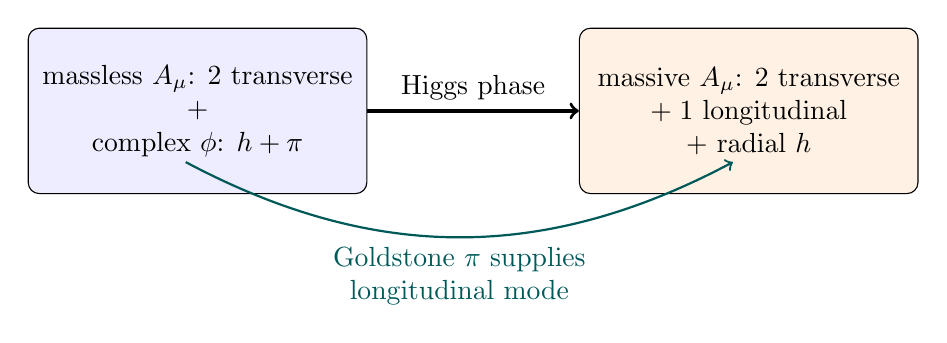
\begin{tikzpicture}[x=1cm,y=1cm]
  \node[draw,rounded corners,fill=blue!7,minimum width=4.3cm,
        minimum height=2.1cm,align=center] (before) at (0,0)
    {massless \(A_\mu\): \(2\) transverse\\
     \(+\)\\
     complex \(\phi\): \(h+\pi\)};
  \node[draw,rounded corners,fill=orange!10,minimum width=4.3cm,
        minimum height=2.1cm,align=center] (after) at (7,0)
    {massive \(A_\mu\): \(2\) transverse\\
     \(+\;1\) longitudinal\\
     \(+\) radial \(h\)};
  \draw[->,very thick] (before) -- node[above]{Higgs phase} (after);
  \draw[->,teal!70!black,thick]
    (-0.15,-0.65) to[bend right=28]
    node[below,align=center]{Goldstone \(\pi\) supplies\\longitudinal mode}
    (6.8,-0.65);
\end{tikzpicture}
\end{adjustbox}
\caption{The Higgs mechanism rearranges, rather than destroys, physical
degrees of freedom.}
\label{fig:l08-degree-rearrangement}
\end{figure}

\begin{classroomqa}
\audiencequestion{How can the angular degree of freedom disappear without
violating degree-of-freedom counting?\lecturetimestamp{01:19:13}}
\lecturerresponse{It does not disappear physically. A massless vector has
two helicities because it cannot be brought to rest. A massive vector has
three polarizations, including a longitudinal one. The Goldstone mode becomes
that third polarization, leaving the total count unchanged.}
\end{classroomqa}

The lecture offers a useful kinematic test. Imagine a vector particle with
mass, slow it to rest, and accelerate it in a new direction. A polarization
that was transverse to the original motion can become longitudinal relative
to the new motion. Likewise, if a circularly polarized massive particle is
carried through rest and sent in the opposite direction, its helicity label
reverses. A strictly massless particle cannot be taken through this
experiment, because no inertial frame can bring it to rest. Its two
helicities therefore form a consistent physical spectrum.

\section{The Superconducting Analogue}

In a conventional superconductor, electrons form Cooper pairs. A pair is a
boson carrying electric charge \(2e\), and the condensate is described by a
charged complex order parameter. When its magnitude is nonzero, the
combination of its phase and the electromagnetic vector potential produces
the Anderson--Higgs mechanism. Static magnetic fields decay over the London
penetration depth rather than extending freely through the bulk. In this
precise medium-dependent sense, the photon behaves as though it has acquired
a mass.

This example also clarifies the opening distinction. The electromagnetic
field is not permanently converted into a different elementary particle.
The massive propagation law belongs to the collective state inside the
material; outside, the vacuum photon remains massless.

\section{What Has Been Established}

The argument can now be compressed without losing its logic:
\begin{enumerate}
  \item A broken global continuous symmetry has a flat angular direction and
        therefore a massless Goldstone mode.
  \item Local phase invariance requires a gauge potential and replaces
        \(\partial_\mu\) by \(D_\mu\).
  \item A bare \(A_\mu A^\mu\) mass violates the local transformation law.
  \item When the charged scalar has nonzero equilibrium magnitude \(f\), the
        gauge-invariant term \(|D_\mu\phi|^2\) contains
        \(\frac12g^2f^2A_\mu A^\mu\).
  \item The phase can be removed by a gauge choice, and its physical degree
        of freedom becomes the longitudinal polarization of the massive
        vector.
  \item The radial Higgs excitation remains, with mass fixed by the curvature
        of the scalar potential.
\end{enumerate}

The next task is to give fermions their masses. Electrons and quarks cannot
use the vector mechanism directly; their Higgs couplings are Yukawa
interactions. Once the scalar settles at \(f\), those interactions become
fermion mass terms.

The broad statement that familiar particles would be massless without
electroweak symmetry breaking requires one final qualification. The
elementary quark and charged-lepton masses, and the \(W\) and \(Z\) masses,
do vanish with the Higgs expectation value. Most of the proton and neutron
mass, however, arises dynamically from QCD confinement and strong-field
energy rather than from the quarks' Higgs masses. That distinction does not
alter the Higgs mechanism derived here; it keeps its domain of application
precise.
